\section{Notação científica. Cargas elétricas}

\frame{
	\frametitle{Notação científica}
	\begin{block}{Definição}
		É uma forma simplificada de representar números reais muito grandes ou muito pequenos nas ciências em geral, por meio do uso de uma potência de base dez.

		$$a \cdot 10^b$$

		onde: \\
		\begin{itemize}
			\item $a$ é chamado de \textbf{mantissa}, ou coeficiente ($1 \leqslant a < 10$).
			\item $b$ é chamado de \textbf{expoente}, ou ordem de grandeza ($b \in \mathbb{Z}$).
		\end{itemize}
	\end{block}
}

\frame{
	\frametitle{Notação científica}
	\begin{block}{Exemplos}
		\begin{itemize}
			\item Raio da terra $ = \SI{6400000}{\meter} = \SI{6.4e6}{\meter} $
			\item $ \num{14000000} = \num{1.4e7} $
			\item $ \num{0.0003} = \num{3e-4} $
		\end{itemize}
	\end{block}
}

\frame{
	\frametitle{Notação científica}
	\begin{block}{Como encontrar a mantissa ou coeficiente?}
		A mantissa, ou coeficiente, é obtida ao \textbf{posicionar a vírgula à direita do primeiro algarismo significativo} do número. Esse reposicionamento da vírgula deve ser feito a partir de divisões ou multiplicações por potências de base dez.
		\begin{itemize}
			\vspace{0.5cm}
			\item A mantissa do número \num{0.00045} é \num{4.5}.
			\item A mantissa do número \num{3256565} é \num{3,256565}.
			\item Por fim, a mantissa, ou coeficiente, do número \num{0,000000003} é $3$.
		\end{itemize}
	\end{block}
}

\frame{
	\frametitle{Notação científica}
	\begin{block}{Como encontrar o expoente ou ordem de grandeza?}
		\begin{itemize}
			\item Se o número a ser escrito na forma de notação científica for decimal, de modo que a \textbf{vírgula tenha de ser deslocada para a direita para encontrar a mantissa}, a \textbf{ordem de grandeza será negativa} e igual ao número de casas decimais que a vírgula deslocou.
			      \vspace{0.5cm}
			\item Caso a \textbf{vírgula precise ser deslocada para a esquerda para encontrar a mantissa}, a \textbf{ordem de grandeza será positiva} e igual ao número de casas decimais que a vírgula deslocou.
		\end{itemize}
	\end{block}
}

\frame{
	\frametitle{Notação científica}
	\begin{block}{Escrevendo em notação científica - Exemplos}
		1 - $0,23$ na forma de notação científica:
		\begin{itemize}
			\item A \textbf{mantissa} é \num{2.3} porque dois é o primeiro algarismo significativo.
			\item Para isso, a vírgula deve ser deslocada uma casa para a direita. Nesse caso, a \textbf{ordem de grandeza} é $-1$.
		\end{itemize}
		\[ \num{0.23} = \num{2.3e-1} \]

		\vspace{0.5cm}

		2 - \num{428000000} na forma de notação científica:
		\begin{itemize}
			\item A \textbf{mantissa} é \num{4,28}.
			\item Para isso, a vírgula deve ser deslocada por oito casas decimais para a esquerda. Assim, a \textbf{ordem de grandeza} é $+8$.
		\end{itemize}
		\[ \num{428000000} = \num{4.28e8} \]
	\end{block}
}

\frame{
	\frametitle{Notação científica}
	\begin{block}{Ajustando a posição da vírgula}
		\begin{gather*}
			\num{25.5e-1}=\num{2.53e0}\\
			\num{0.0063e5}=\num{6.3e2}	
		\end{gather*}
	\end{block}
}

\frame{
	\frametitle{Notação científica}
	\begin{block}{Operações básicas - Soma e subtração - Exemplos}
		\begin{itemize}
			\item Deve-se igualar os expoentes.
		\end{itemize}
		
		\begin{gather*}
			\num{1.8e2} + \num{2.4e3} = \num{1.8e2} + \num{24e2} = \num{25.8e2} = \num{2.58e3}\\[2em]
			\num{6.4e4} - \num{2.0e3} = \num{64e3} - \num{2.0e3} = \num{62e3} = \num{6.2e4}
		\end{gather*}
	\end{block}
}

\frame{
	\frametitle{Notação científica}
	\begin{block}{Operações básicas - Multiplicação e divisão - Exemplos}
		\begin{gather*}
			\num{6.0e3}\times\num{3.0e8} = \num{18e11} = \num{1.8e12}\\[2em]
			\num{6.0e3}\div\num{3.0e8} = \num{2e-5}
		\end{gather*}
	\end{block}
}

\frame{
	\frametitle{Notação científica}
	\begin{block}{Operações básicas - Potência e raiz - Exemplos}
		\begin{itemize}
			\item Deve-se elevar o coeficiente e multiplicar o expoente.
		\end{itemize}
	
		\begin{gather*}
			(\num{3.0e2})^2 = \num{3.0}^2 \cdot (10^{2})^2 = \num{9e4}\\[2em]
			\sqrt{\num{36e4}} = (\num{36e4})^{1/2} = \num{6e2}
		\end{gather*}
	\end{block}
}

\frame{
	\frametitle{Cargas elétricas}
	\begin{block}{Introdução}
		\begin{itemize}
			\item Toda a matéria que conhecemos é formada por moléculas. Esta, por sua vez, é formada de átomos, que são compostos por três tipos de partículas elementares: prótons, nêutrons e elétrons.
			\item Os átomos são formados por um núcleo, onde ficam os prótons e nêutrons e uma eletrosfera, onde os elétrons permanecem, em órbita.
			\item Os prótons e nêutrons têm massa praticamente igual, mas a massa dos elétrons é aproximadamente 2 mil vezes menor que a massa dos prótons.
		\end{itemize}
	\end{block}
}

\frame{
	\frametitle{Cargas elétricas}
	\centerline{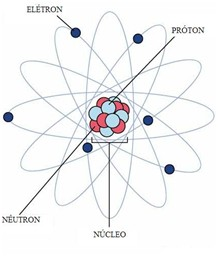
\includegraphics[width=0.5\linewidth]{Figuras/Ch02/atomo.jpg}}
}

\frame{
	\frametitle{Cargas elétricas}
	\begin{block}{Propriedade}
		\begin{itemize}
			\item Se pudéssemos separar os prótons, nêutrons e elétrons de um átomo, e lançá-los em direção à um ímã, os prótons seriam desviados para uma direção, os elétrons a uma direção oposta a do desvio dos prótons, e os nêutrons não seriam afetados.
			\item Esta propriedade de cada uma das partículas é chamada \textbf{carga elétrica} (unidade no SI: coulomb [\si{\coulomb}]). Os prótons são partículas com cargas \textbf{positivas}, os elétrons tem carga \textbf{negativa} e os nêutrons tem carga \textbf{neutra}.
		\end{itemize}
	\end{block}

	\centerline{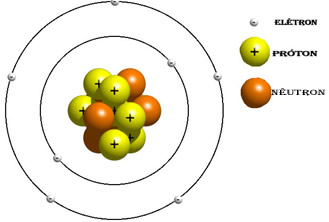
\includegraphics[width=0.4\linewidth]{Figuras/Ch02/atomo2.jpg}}
}

\frame{
	\frametitle{Cargas elétricas}
	\begin{block}{Carga elétrica elementar}
		\begin{itemize}
			\item Um próton e um elétron têm valores absolutos iguais, embora tenham sinais opostos. O valor da carga de um próton ou um elétron é chamado carga elétrica elementar e simbolizado por $\bm{e}$.
			\item A carga elétrica elementar é a menor quantidade de carga encontrada na natureza, comparando-se este valor com coulomb, têm-se a relação:
		\end{itemize}
		
		\begin{align*}
			\text{prótons} &\implies e = \SI{1.6e-19}{\coulomb}\\
			\text{elétrons} &\implies e = \SI{-1.6e-19}{\coulomb}
		\end{align*}
	\end{block}
}

\frame{
	\frametitle{Cargas elétricas}
	\begin{block}{Carga elétrica}
		O módulo da carga elétrica pode ser definido como:
		$$\boxed{Q = n \cdot e}$$
		onde $n$ é o número de cargas elementares.
	\end{block}
}

\frame{
	\frametitle{Cargas elétricas}
	\begin{block}{Conclusão}
		\begin{itemize}
			\item Se um corpo está com \textbf{carga elétrica positiva} existe uma falta de elétrons, assim o número de prótons é maior que o número de elétrons.
			      \vspace{0.5cm}
			\item Se um corpo está com \textbf{carga elétrica negativa} existe uma falta de prótons, assim o número de prótons é menor que o número de elétrons.
			      \vspace{0.5cm}
			\item Se um corpo está com \textbf{carga elétrica neutra}, o número de prótons é igual ao número de elétrons.
		\end{itemize}
	\end{block}
}

\frame{
	\frametitle{Atração e repulsão}
	
	\setmyunit{1.5cm}
	
	\centering
	\begin{tikzpicture}
		\draw (0,0) circle (0.25) node[] {P} (2,0) circle (0.25) node[] {e}
			(0.5,-1) circle (0.25) node[] {P} (1.5,-1) circle (0.25) node[] {P}
			(0.5,-2) circle (0.25) node[] {e} (1.5,-2) circle (0.25) node[] {e}
			(0.25,-3) circle (0.25) node[] {N} (1.75,-3) circle (0.25) node[] {N};
		\draw[-Latex] (0.25,0) -- +(0.25,0);
		\draw[-Latex] (1.75,0) -- +(-0.25,0);
		\node at (1,-0.4) {Atraem-se};
		\draw[-Latex] (0.25,-1) -- +(-0.25,0);
		\draw[-Latex] (1.75,-1) -- +(0.25,0);
		\node at (1,-1.5) {Repelem-se};
		\draw[-Latex] (0.25,-2) -- +(-0.25,0);
		\draw[-Latex] (1.75,-2) -- +(0.25,0);
		\node at (1,-2.5) {Repelem-se};
		
		\node at (1,-3.5) {Não há interação de campo};
	\end{tikzpicture}
	
%	\centerline{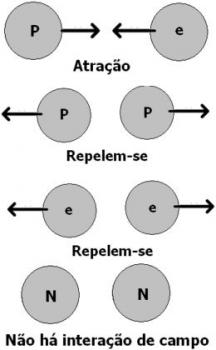
\includegraphics[width=0.4\linewidth]{Figuras/Ch02/atracao.jpg}}
}

\frame{
	\frametitle{Classificação dos materiais}
	\begin{block}{Definição}
		Cotidianamente estamos em contato com elementos que são condutores elétricos e outros que são isolantes elétricos. O que diferencia esses elementos, permitindo que uns possuam maior facilidade de conduzir eletricidade do que outros, é a estrutura atômica de cada substância.
	\end{block}

\bigskip
	\centerline{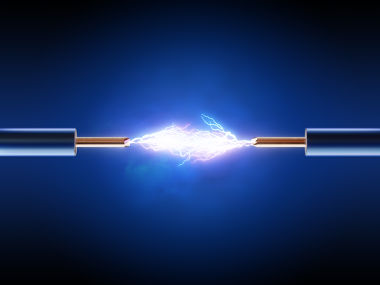
\includegraphics[width=0.4\linewidth]{Figuras/Ch02/condutores.jpg}}
}

\frame{
	\frametitle{Classificação dos materiais}
	\begin{block}{Condutores}
		\begin{itemize}
			\item Os corpos considerados condutores elétricos possuem excesso de elétrons em sua camada de valência, que é a última camada a receber elétrons em um átomo.
			\item Os elétrons presentes na camada de valência são denominados de elétrons livres, e a força de atração entre eles e o núcleo atômico é pequena, logo, eles possuem facilidade de se movimentar pelo material, tornando a substância em questão um bom condutor de eletricidade.
		\end{itemize}
	\end{block}
	\centerline{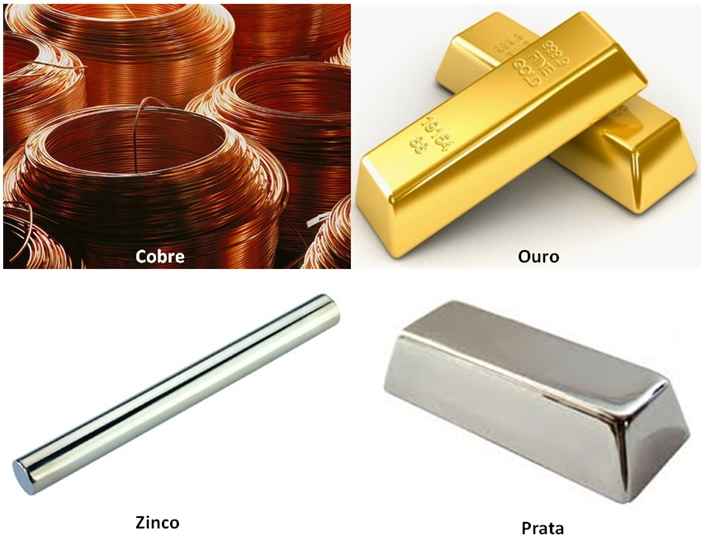
\includegraphics[width=0.37\linewidth]{Figuras/Ch02/condutores2.jpg}}
}

\frame{
	\frametitle{Classificação dos materiais}
	\begin{block}{Isolantes}
		\begin{itemize}
			\item Eles são também chamados de dielétricos.
			\item Os elétrons que formam esses materiais não têm facilidade de movimentação, tendo em vista a forte ligação entre eles e o núcleo atômico.
		\end{itemize}
	\end{block}

	\bigskip
	
	\centerline{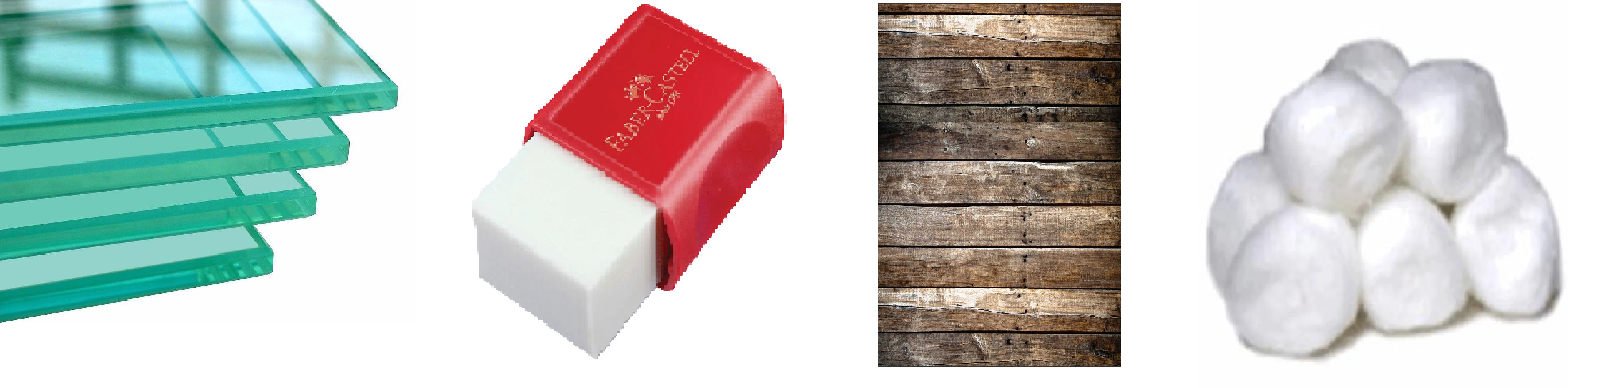
\includegraphics[width=0.8\linewidth]{Figuras/Ch02/isolantes.png}}
}

\frame{
	\frametitle{Classificação dos materiais}
	\begin{block}{Semicondutores}
		\begin{itemize}
			\item Os materiais denominados de semicondutores possuem propriedades elétricas intermediárias entre condutores e isolantes.
			\item As condições físicas às quais o material é submetido determinam se ele se comportará como condutor ou como um isolante. Esses materiais são largamente utilizados pela indústria de eletrônicos para a composição de circuitos.
		\end{itemize}
	\end{block}
	\centerline{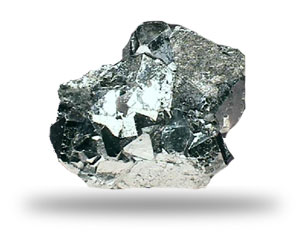
\includegraphics[width=0.4\linewidth]{Figuras/Ch02/silicio.jpg}}
}

\section*{Exercícios}

\frame{
	\frametitle{Exercícios}
	\begin{block}{}
		01. A respeito da condutividade elétrica e térmica dos materiais, marque a alternativa correta:

		\vspace{0.5cm}

		(a) Somente os metais podem conduzir eletricidade e calor.

		\vspace{0.3cm}

		(b) Em hipótese alguma, um dielétrico pode conduzir corrente elétrica ou calor.

		\vspace{0.3cm}

		(c) Os metais destacam-se como bons condutores elétricos porque possuem excesso de prótons em sua estrutura atômica.

		\vspace{0.3cm}

		(d) Os materiais que são isolantes elétricos possuem alta condutividade elétrica.

		\vspace{0.3cm}

		(e) Um material é melhor condutor que outro quando possuir valor de condutividade elétrica maior.
	\end{block}
}

\section*{Referências}

\frame{
	\frametitle{Referências e Exercícios Complementares}
	\begin{itemize}
		\item Física, Ciência e Tecnologia – Vol 3. PENTEADO, Paulo César M; TORRES, Carlos Magno A. Ed. Moderna (2006)
	\end{itemize}
	%\centering{\alert{Página 36 - \textbf{1.6.1 até 1.6.5, 1.6.17 até 1.6.19}}} \\
	%https://www.youtube.com/watch?v=IUgS7Uw-qBI
	\centering{\alert{Lista de exercícios 02}}
}